\ifx\wholebook\relax\else
% --------------------------------------------
% Lulu:
    \documentclass[a4paper,12pt,twoside]{../includes/ThesisStyle}

	\usepackage[T1]{fontenc} %%%key to get copy and paste for the code!
%\usepackage[utf8]{inputenc} %%% to support copy and paste with accents for frnehc stuff
\usepackage{times}
\usepackage{ifthen}
\usepackage{xspace}
\usepackage{alltt}
\usepackage{latexsym}
\usepackage{url}            
\usepackage{amssymb}
\usepackage{amsfonts}
\usepackage{amsmath}
\usepackage{stmaryrd}
\usepackage{enumerate}
\usepackage{cite}
%\usepackage[pdftex,colorlinks=true,pdfstartview=FitV,linkcolor=blue,citecolor=blue,urlcolor=blue]{hyperref}
\usepackage{xspace}
%\usepackage{graphicx}
\usepackage{subfigure}
\usepackage[scaled=0.85]{helvet}
        
        
\newcommand{\sepe}{\mbox{>>}}
\newcommand{\pack}[1]{\emph{#1}}
\newcommand{\ozo}{\textsc{oZone}\xspace}
\newcommand\currentissues{\par\smallskip\textbf{Current Issues -- }}

\newboolean{showcomments}
\setboolean{showcomments}{true}
\ifthenelse{\boolean{showcomments}}
  {\newcommand{\bnote}[2]{
	\fbox{\bfseries\sffamily\scriptsize#1}
    {\sf\small$\blacktriangleright$\textit{#2}$\blacktriangleleft$}
    % \marginpar{\fbox{\bfseries\sffamily#1}}
   }
   \newcommand{\cvsversion}{\emph{\scriptsize$-$Id: macros.tex,v 1.1.1.1 2007/02/28 13:43:36 bergel Exp $-$}}
  }
  {\newcommand{\bnote}[2]{}
   \newcommand{\cvsversion}{}
  } 


\newcommand{\here}{\bnote{***}{CONTINUE HERE}}
\newcommand{\nb}[1]{\bnote{NB}{#1}}
\newcommand{\fix}[1]{\bnote{FIX}{#1}}
%%%% add your own macros 

\newcommand{\sd}[1]{\bnote{Stef}{#1}}
\newcommand{\ja}[1]{\bnote{Jannik}{#1}}
\newcommand{\na}[1]{\bnote{Nico}{#1}}
%%% 


\newcommand{\figref}[1]{Figure~\ref{fig:#1}}
\newcommand{\figlabel}[1]{\label{fig:#1}}
\newcommand{\tabref}[1]{Table~\ref{tab:#1}}
\newcommand{\layout}[1]{#1}
\newcommand{\commented}[1]{}
\newcommand{\secref}[1]{Section \ref{sec:#1}}
\newcommand{\seclabel}[1]{\label{sec:#1}}

%\newcommand{\ct}[1]{\textsf{#1}}
\newcommand{\stCode}[1]{\textsf{#1}}
\newcommand{\stMethod}[1]{\textsf{#1}}
\newcommand{\sep}{\texttt{>>}\xspace}
\newcommand{\stAssoc}{\texttt{->}\xspace}

\newcommand{\stBar}{$\mid$}
\newcommand{\stSelector}{$\gg$}
\newcommand{\ret}{\^{}}
\newcommand{\msup}{$>$}
%\newcommand{\ret}{$\uparrow$\xspace}

\newcommand{\myparagraph}[1]{\noindent\textbf{#1.}}
\newcommand{\eg}{\emph{e.g.,}\xspace}
\newcommand{\ie}{\emph{i.e.,}\xspace}
\newcommand{\ct}[1]{{\textsf{#1}}\xspace}


\newenvironment{code}
    {\begin{alltt}\sffamily}
    {\end{alltt}\normalsize}

\newcommand{\defaultScale}{0.55}
\newcommand{\pic}[3]{
   \begin{figure}[h]
   \begin{center}
   \includegraphics[scale=\defaultScale]{#1}
   \caption{#2}
   \label{#3}
   \end{center}
   \end{figure}
}

\newcommand{\twocolumnpic}[3]{
   \begin{figure*}[!ht]
   \begin{center}
   \includegraphics[scale=\defaultScale]{#1}
   \caption{#2}
   \label{#3}
   \end{center}
   \end{figure*}}

\newcommand{\infe}{$<$}
\newcommand{\supe}{$\rightarrow$\xspace}
\newcommand{\di}{$\gg$\xspace}
\newcommand{\adhoc}{\textit{ad-hoc}\xspace}

\usepackage{url}            
\makeatletter
\def\url@leostyle{%
  \@ifundefined{selectfont}{\def\UrlFont{\sf}}{\def\UrlFont{\small\sffamily}}}
\makeatother
% Now actually use the newly defined style.
\urlstyle{leo}


	
	\usepackage{amsmath,amssymb}             % AMS Math
% \usepackage[french]{babel}
\usepackage[latin1]{inputenc}
\usepackage[T1]{fontenc}
\usepackage[left=1.5in,right=1.3in,top=1.1in,bottom=1.1in,includefoot,includehead,headheight=13.6pt]{geometry}
\renewcommand{\baselinestretch}{1.05}

\usepackage{multicol}

% Table of contents for each chapter

\usepackage[nottoc, notlof, notlot]{tocbibind}
\usepackage{minitoc}
\setcounter{minitocdepth}{1}
\mtcindent=15pt
% Use \minitoc where to put a table of contents

\usepackage{enumitem}

\usepackage{aecompl}

% Glossary / list of abbreviations

%\usepackage[intoc]{nomencl}
%\renewcommand{\nomname}{List of Abbreviations}
%
%\makenomenclature

% My pdf code

\usepackage[pdftex]{graphicx}
\usepackage[a4paper,pagebackref,hyperindex=true]{hyperref}

\usepackage{pgfplotstable,booktabs,colortbl}
\pgfplotsset{compat=1.8}

% Links in pdf
\usepackage{color}
\definecolor{linkcol}{rgb}{0,0,0.4} 
\definecolor{citecol}{rgb}{0.5,0,0} 

% Change this to change the informations included in the pdf file

% See hyperref documentation for information on those parameters

\hypersetup
{
bookmarksopen=true,
pdftitle="Sista: a Metacircular Architecture for Runtime Optimisation Persistence",
pdfauthor="Clement BERA", 
pdfsubject="Thesis", %subject of the document
%pdftoolbar=false, % toolbar hidden
pdfmenubar=true, %menubar shown
pdfhighlight=/O, %effect of clicking on a link
colorlinks=true, %couleurs sur les liens hypertextes
pdfpagemode=None, %aucun mode de page
pdfpagelayout=SinglePage, %ouverture en simple page
pdffitwindow=true, %pages ouvertes entierement dans toute la fenetre
linkcolor=linkcol, %couleur des liens hypertextes internes
citecolor=citecol, %couleur des liens pour les citations
urlcolor=linkcol %couleur des liens pour les url
}

% definitions.
% -------------------

\setcounter{secnumdepth}{3}
\setcounter{tocdepth}{1}

% Some useful commands and shortcut for maths:  partial derivative and stuff

\newcommand{\pd}[2]{\frac{\partial #1}{\partial #2}}
\def\abs{\operatorname{abs}}
\def\argmax{\operatornamewithlimits{arg\,max}}
\def\argmin{\operatornamewithlimits{arg\,min}}
\def\diag{\operatorname{Diag}}
\newcommand{\eqRef}[1]{(\ref{#1})}

\usepackage{rotating}                    % Sideways of figures & tables
%\usepackage{bibunits}
%\usepackage[sectionbib]{chapterbib}          % Cross-reference package (Natural BiB)
%\usepackage{natbib}                  % Put References at the end of each chapter
                                         % Do not put 'sectionbib' option here.
                                         % Sectionbib option in 'natbib' will do.
\usepackage{fancyhdr}                    % Fancy Header and Footer

% \usepackage{txfonts}                     % Public Times New Roman text & math font
  
%%% Fancy Header %%%%%%%%%%%%%%%%%%%%%%%%%%%%%%%%%%%%%%%%%%%%%%%%%%%%%%%%%%%%%%%%%%
% Fancy Header Style Options

\pagestyle{fancy}                       % Sets fancy header and footer
\fancyfoot{}                            % Delete current footer settings

%\renewcommand{\chaptermark}[1]{         % Lower Case Chapter marker style
%  \markboth{\chaptername\ \thechapter.\ #1}}{}} %

%\renewcommand{\sectionmark}[1]{         % Lower case Section marker style
%  \markright{\thesection.\ #1}}         %

\fancyhead[LE,RO]{\bfseries\thepage}    % Page number (boldface) in left on even
% pages and right on odd pages
\fancyhead[RE]{\bfseries\nouppercase{\leftmark}}      % Chapter in the right on even pages
\fancyhead[LO]{\bfseries\nouppercase{\rightmark}}     % Section in the left on odd pages

\let\headruleORIG\headrule
\renewcommand{\headrule}{\color{black} \headruleORIG}
\renewcommand{\headrulewidth}{1.0pt}
\usepackage{colortbl}
\arrayrulecolor{black}

\fancypagestyle{plain}{
  \fancyhead{}
  \fancyfoot{}
  \renewcommand{\headrulewidth}{0pt}
}

\usepackage{algorithm}
\usepackage[noend]{algorithmic}

%%% Clear Header %%%%%%%%%%%%%%%%%%%%%%%%%%%%%%%%%%%%%%%%%%%%%%%%%%%%%%%%%%%%%%%%%%
% Clear Header Style on the Last Empty Odd pages
\makeatletter

\def\cleardoublepage{\clearpage\if@twoside \ifodd\c@page\else%
  \hbox{}%
  \thispagestyle{empty}%              % Empty header styles
  \newpage%
  \if@twocolumn\hbox{}\newpage\fi\fi\fi}

\makeatother
 
%%%%%%%%%%%%%%%%%%%%%%%%%%%%%%%%%%%%%%%%%%%%%%%%%%%%%%%%%%%%%%%%%%%%%%%%%%%%%%% 
% Prints your review date and 'Draft Version' (From Josullvn, CS, CMU)
\newcommand{\reviewtimetoday}[2]{\special{!userdict begin
    /bop-hook{gsave 20 710 translate 45 rotate 0.8 setgray
      /Times-Roman findfont 12 scalefont setfont 0 0   moveto (#1) show
      0 -12 moveto (#2) show grestore}def end}}
% You can turn on or off this option.
% \reviewtimetoday{\today}{Draft Version}
%%%%%%%%%%%%%%%%%%%%%%%%%%%%%%%%%%%%%%%%%%%%%%%%%%%%%%%%%%%%%%%%%%%%%%%%%%%%%%% 

\newenvironment{maxime}[1]
{
\vspace*{0cm}
\hfill
\begin{minipage}{0.5\textwidth}%
%\rule[0.5ex]{\textwidth}{0.1mm}\\%
\hrulefill $\:$ {\bf #1}\\
%\vspace*{-0.25cm}
\it 
}%
{%

\hrulefill
\vspace*{0.5cm}%
\end{minipage}
}

\let\minitocORIG\minitoc
\renewcommand{\minitoc}{\minitocORIG \vspace{1.5em}}

\usepackage{multirow}
\usepackage{slashbox}

\newenvironment{bulletList}%
{ \begin{list}%
	{$\bullet$}%
	{\setlength{\labelwidth}{25pt}%
	 \setlength{\leftmargin}{30pt}%
	 \setlength{\itemsep}{\parsep}}}%
{ \end{list} }

\newtheorem{definition}{D�finition}
\renewcommand{\epsilon}{\varepsilon}

% centered page environment

\newenvironment{vcenterpage}
{\newpage\vspace*{\fill}\thispagestyle{empty}\renewcommand{\headrulewidth}{0pt}}
{\vspace*{\fill}}



	\graphicspath{{.}{../figures/}}
	\begin{document}
\fi

\chapter{Test architecture}
\label{chap:tests}
\minitoc

In this work, there is a clear distinction between the runtime bytecode to bytecode optimiser, implemented in Smalltalk, and bytecode to machine code back-end, implemented in Slang. Both entites are entirely separated relying on the specified interface between the VM and the image to communicate.

As for many projects, to limit the number of bugs and to increase the overall quality of the project, we added automated tests. Such tests are performed automatically by the continuous integration server to validate new commits.

Because of the split by design, it was possible to test separatedly the runtime bytecode to bytecode optimiser and the back-end. Testing both parts separatedly ease the development process, as a failing test one part requires the programmer to look for bug only in this part of the code. In addition, it enables testing technique hardly possible otherwise, as the symbolic execution experiment detailled in one of the next subsection.

\section{Runtime optimiser tests}

\subsection{Test framework: inputs and passes}

optimizer used statically.

Validator thing

- methods
- opt passes
- what to validate

graph sanity and co

\subsection{Testing context to context deoptimisation}

deopt split in 2, test both separatedly. => each interrupt point on set of methods.

\subsection{Experimental symbolic execution}

Doc: paper tests + TODO.

\section{Back-end tests}

The bytecode to machine code back-end was already in production as the baseline JIT on multiple processors (x86, x64, ARMv6). As we are conceptually reusing the same component, it should be stable. However, the runtimer optimiser produces bytecode from the extended bytecode set not present in the baseline JIT, requires non optimised code to be compiled with counters for hot spot detection and uses machine code introspection to read inline cache data. These aspects needs to be tested separatedly. 

\subsection{Extended bytecode set tests}

The bytecode set was extended so the runtime compiler can generate bytecode using unsafe operations, such as array access without bound checks. These operations needs to be tested. 

To perform the tests, a virtual machine with support for the runtime compiler was compiled. However, all the Smalltalk code was annotated before the tests as code that cannot be optimised. This way, the runtime optimiser is never triggered and no optimised code is ever present. As non of the code is optimised, the Smalltalk runtime works perfectly using only the part of the back-end which is production ready.

In this context, it is possible to generate new compiled code, manually writting a specific sequence of bytecode in it, execute it and ensure that the runtime has not crashed and that the result is as expected. 

\paragraph{Less or equal example.} One of the unsafe operation is called \emph{USmiLessOrEqual}. This operation is equivalent to the operation \ct{<=}, but expects both operands to be instances of \ct{SmallInteger} (signed 31-bits tagged integers), else the behavior is undefined. It is normally used by the optimiser only when it can ensure that the two operands are instances of \ct{SmallInteger}.

\paragraph{Less or equal example: what to test.}

To test USmiLessOrEqual, one could take important range of integers and check that the result of each integer against each other integer within the range would give the correct answer. This approach looks nice, but it does not really test eficiently the back-end. The implementation of USmiLessOrEqual forwards to the C operation <= for integers in the interpreter, and to the CPU instructions compare then jumpBelowOrEqual/jumpGreater in the JIT compiler. Hence, by testing a range of integers, one would actually test if the C operation <= for integers or the processor opcodes for comparison and branching actually works. That's not the goal.

However, the interpretation of the code and the machine code generated by the JIT compiler needs to be correct for USmiLessOrEqual. In addition, for coverage, all the different branches needs to be taken. For example, all the possible branches used to generate machine code for USmiLessOrEqual in the code of the JIT compiler as well as all the branches that can be taken at runtime in the generated machine code need to be tested.

How many possible branches there are when executing the code that performs the operation USmiLessOrEqual with two operands a and b ? Let's discuss the different branches in the JIT compiler and machine code generated. The interpreter has only a subset of those cases.

Pseudo-code:

\ct{a USmiLessOrEqual: b}

Bytecode:

\begin{code}
pushTemp: 0
pushTemp: 1
callPrimitive: \#USmiLessOrEqual
\end{code}

The operation expects the two operands to be integers. This is ensured by the runtime optimizer, and the behavior when a or b is not an integer is undefined, so one does not need to test the cases where a or b is not a SmallInteger. For the rest of this section, we assume that the two operands are SmallIntegers.

One could think there are actually two cases for this operation (we will call them cases A):

Case A1: a <= b, so the operation should answer true.

Case A2: a > b, so the operation should answer false.

These two cases will definitely answer different results, they will definitely take two different paths in the virtual machine (one path pushing true on stack, the other pushing false) so they need both to be tested. But that is more complex: if the operation USmiLessOrEqual is directly followed by a branchTrue or a branchFalse, the JIT compiler generates different machine code to quicken the branch execution.

The machine code for \ct{a USmiLessOrEqual: b}, if not followed by a branch, looks like that:

\begin{code}
cpu compare: a with: b
cpu jumpBelowOrEqual:
cpu push: false
cpu jump:
cpu push: true
...
\end{code}

There is already a branch in the machine code, with one path pushing true and one path pushing false on the stack.

The machine code for \ct{a branchFalse} for example looks like that:

cpu compare: a with: false
cpu jumpEqual: (jump to false branch )
cpu compare: a with: true
cpu jumpEqual: (jump to true branch )
cpu callMustBeBooleanTrampoline
(code for false branch)
...
cpu jump: (jump over true branch)
(code for true branch)
...

There are three possible paths for a normal branch, depending on if a is true, false or a non boolean.

The JIT quickens the branch by directly using the branches of USmiLessOrEqual and not generating the push booleans as well as the comparison between booleans and true and false. USmiLessOrEqual answers true or false, so there is no need to compile the mustBeBoolean fall back. The generated code for: \ct{(a USmiLessOrEqual: b) branchTrue} will then look like that:

cpu compare: a with: b
cpu jumpBelowOrEqual: (jump to true branch)
(code for false branch)
...
cpu jump: (jump over true branch)
(code for true branch)
...

Three cases are defined (we will call them cases B), depending on what follows USmiLessOrEqual:

Case B1 (no branch):
a USmiLessOrEqual: b

Case B2 (branchTrue):
(a USmiLessOrEqual: b) ifTrue: [ "some code" ]

Case B3 (branchFalse):
(a USmiLessOrEqual: b) ifFalse: [ "some code" ]

Cases A combined with cases B means that for the operation USmiLessOrEqual, we have 6 (2 * 3) different possibles cases to be tested.

In addition, the JIT compiler has to generate heavily optimized code (by carefully selecting the native instructions to generate) for unsafe operations as they are present in optimised methods which are frequently used. Instruction selection depends on the state of the JIT's simulated stack, \ie if one of the operand is a SmallInteger literal. SmallInteger instances answer specific properties: they're immutable and cannot be become, making them suitable for compiler optimisations.

pushTemp: 0
pushTemp: 1
callPrimitive: USmiLessOrEqual

The pushTemp: operations have generated in the JIT compiler code to put the operands in registers or to spill them on stack as they are temporary variable. If the variable was a cpu constant, it would have just remembered the value and will generate the code for the cpu constant only when the constant will be used. For this operation, both operands are necessarily cpu variables. If one operand is a constant, the JIT will generate a native instruction comparing a constant versus a register, else it will generate a native instruction comparing two registers.

The JIT compiler distinguishes 3 different operations at compilation time for USmiLessOrEqual:

Case C1: a is a cpu constant and b is a cpu variable

Case C2: a is a cpu variable and b is a cpu constant

Case C3: a is a cpu variable and b is a cpu variable

The JIT compiler backend assumes that if both operands are cpu constants, the operation would have been statically computed by the optimiser at compilation time. The operation would still work, it would just be optimized as if one of the operand was a cpu variable (putting one of the constant into a register first).

This means that in the machine code for USmiLessOrEqual, one has to test 18 cases (Cases A combined with cases B combined with cases C).

\paragraph{Less or equal example: testing all the cases.}
(Rewrite this section)

For convenience, I am going to test this instruction image-side and not VM-side.

To test each case, I need to have a compiled method with the bytecode sequence I want to test. For example, I may want a sequence such as the two operands are cpu variables (not cpu constants) and the operation USmiLessOrEqual is followed by a branchTrue.

To do that, I created a method to instrument. Let's look at its code:

methodToInstrument
"This method is instrumented in the tests. Do *not* edit it.

The instrumentation starts after the last temporary assignment.
Temporaries are result of message sends, so they're in registers
or spilled on stack, whereas literals are constants.

Code after the last temporary assignment is here to generate the
required literals and to let enough room in the bytecode zone of
the method for instrumentation."

\begin{code}
| t50 t3 tArray tByteArray |
t50 := self get50.
t3 := self get3.
tArray := self getArray.
tByteArray := self getByteArray.
5 + 10 + #(1 2 3 4 5 6) first + #[1 2 3 4 5 6 7 8] first.
^ t3 + t50 + t3 + t50 + t3 + t50 + t3 + t50 + t3 + t50
\end{code}

In different tests, I will need 2 different integer constants, a byteArray and an Array in register or spilled on stack. This is why the method start by getting into temporary variables such values. The byteArray and the array are used in other tests than the one of USmiLessOrEqual. They are used for tests on variable object access unsafe operations. I will not detail them here.

Let's look quickly into the methods called:

\begin{code}
get3
^ 3

get50
^ 50

getArray
^ #( 1 2 3 4 5 6 7 8 9 10 11)

getByteArray
^ #[ 1 2 3 4 5 6 7 8 9]
\end{code}

As explained in the method comments, the method will be instrumented after the last temporary assignment, in order to be able to use the values in temporary in the generated code.

Based on the original method's code, I know that at the point where method instrumentation will start:

temporary variable number 0, t50, holds 50
temporary variable number 1, t3, holds 3
temporary variable number 2, tArray holds \#( 1 2 3 4 5 6 7 8 9 10 11)
temporary variable number 3, tByteArray holds \#[ 1 2 3 4 5 6 7 8 9]
literal number 0 holds 5
literal number 1 holds 10
literal number 2 holds \#(1 2 3 4 5 6)
literal number 3 holds \#[1 2 3 4 5 6 7 8]
The difference between values held by the literals and the ones held in temporary variables is that values held by the literals will be compiled into cpu constants, whereas values held by the temporary variables will be compiled either into an assignment to a register or spilled on stack.

Based on my knowledge on the current state of the method, I am going to use specific methods to generate the code I want. For example, if I want to generate the constant 5, I am going to use:

genCst5: encoder
encoder genPushLiteral: 4

Now that I have everything at hand, let's instrument the method. First I need to generate the bytecodes I want. I use a simple pattern (which may not be very well designed) where I hold in an array all the possible cases and the expected value. For USmiLessOrEqual, it's cases description gives you:

1) Possible pairs of operands that answers true to USmiLessOrEqual (cases C, operands are cpu constants or not, I added a cases with 2 cpu constants as operands just in case):
\{ self blockGenVar3 . self blockGenVar50 \} .
\{ self blockGenVar3 . self blockGenCst5 \} .
\{ self blockGenCst5 . self blockGenVar50 \} .
\{ self blockGenCst5 . self blockGenCst10 \}

2) This is combined with the possible results answered (Cases A). Basically I will check that operand1 USmiLessOrEqual: operand2 answers true, and the opposite, operand2 USmiLessOrEqual: operand1 answers false:
\{ self blockGenSuccessively: truePair . true \} .
\{ self blockGenSuccessively: (self invertedPair: truePair) . false \}

3) Lastly I combined them with possibility of being followed by branches. For this purpose I used branches that push different integers on stack to check the result. For instance:

\begin{code}
jumpFalse10Else5Block
^ [ :encoder |
encoder genBranchPopFalse: 2.
self genCst5: encoder.
encoder genJump: 1.
self genCst10: encoder. ]
\end{code}

Here, if value on stack is true, there will be 5 on stack after the branch, else there will be 10. This bytecode sequence is equivalent to ifTrue: [ 5 ] ifFalse: [ 10] with the receiver of ifTrue:ifFalse: on stack.

Here are the different branch cases to combine (cases B), first arg is the block that generates or not the branch, the other is the expected result:
int := self jumpBlockResult: boolean.
\{ self emptyBlock . boolean \} .
\{ self jumpFalse10Else5Block . int \} .
\{ self jumpTrue5Else10Block . int \}

Ok. So for USmiLessOrEqual, we are going to generate 24 (2 * 3 * 4) bytecode sequences to test. Let's generate the first one:

The two operands are in registers or spilled on stack{ self blockGenVar3 . self blockGenVar50 }
The result of the operation will be true (3 <= 50)
The operation is not followed by a branch
I get the bytecode sequence:
65 pushTemp: 1 "holds 3"
64 pushTemp: 0 "holds 50"
248 243 7 callInlinedPrimitive: USmiLessOrEqual
92 ReturnTop

Note that we added a returnTop at the end to be sure that the method will return the result to test afterwards. We cannot let the original bytecode that remains in the compiled method be executed after our hand-written bytecodes.

\begin{figure}[!htp]
\begin{center}
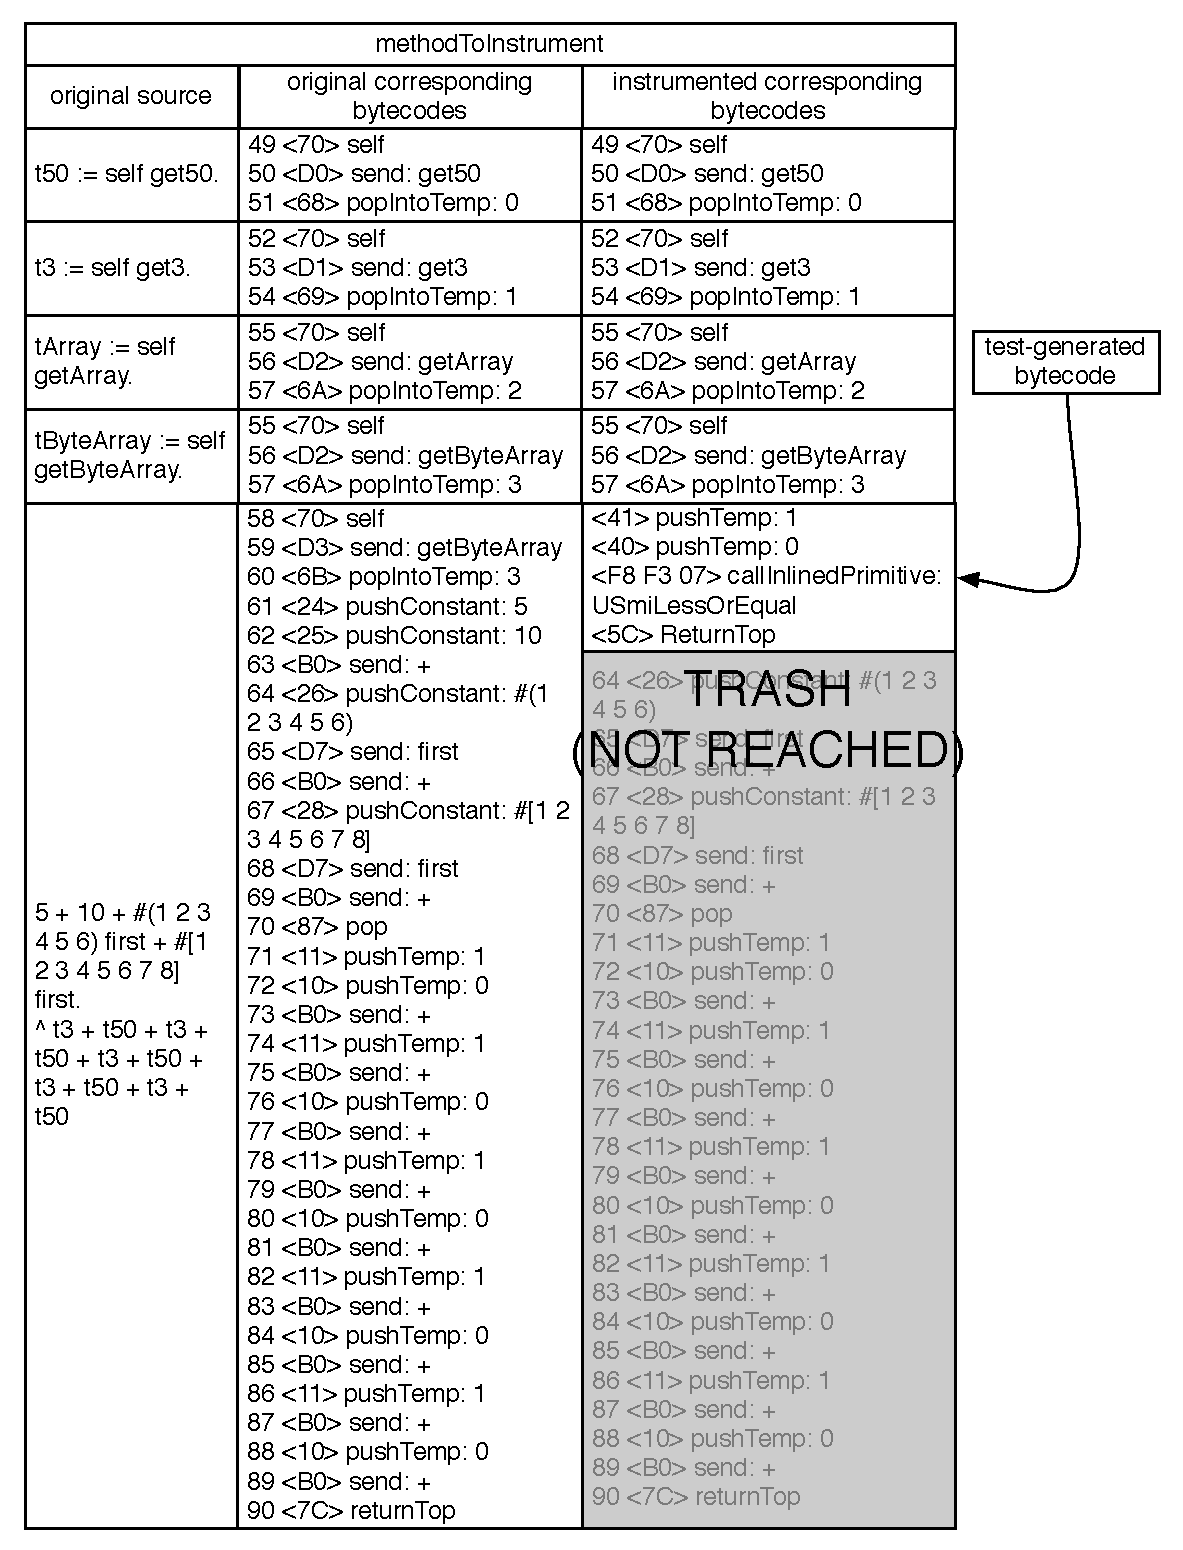
\includegraphics[width=1.0\linewidth]{methodInstrumentation}
\caption{Method instrumentation}
\figlabel{methodInstrumentation}
\end{center}
\end{figure}

On \figref{methodInstrumentation}, on the left is the original source code and bytecodes of the method. After the last temporary assignment, we override the bytecodes and write down our bytecode sequence. We use an instrumented method that is long enough so there is enough room to correctly write down the test-generated bytecode.

Then, we need to void the method Cog VM state. The method may already be compiled to machine code with another bytecode sequence (from the previous tests for example, as they are typically all run in a row). Voiding the Cog VM state asks the VM to flush its machine code state for the method to flush this kind of dependencies.

method voidCogVMState

Now we can run the method. I run it several times to have both the interpreter and the machine code results:

\begin{code}
runInstrumentedMethod
| res |
res := { nil . nil }.
res at: 1 put: self runMethodToInstrument. "interpreter result"
1 to: 5 do: [ :i | self runMethodToInstrument ]. "heat up the JIT"
res at: 2 put: self runMethodToInstrument. "jitted result"
^ res
\end{code}

Lastly, I can compare the two results I collected from the runtime to the expected result. The operation USmiLessOrEqual is fully tested .

\paragraph{Discussion.} Now, one needs to understand that such tests are not safe: if the test fails, sometimes one will just have an assertion failure, but in most cases one has a segmentation fault to debug in the VM simulator. I could run the test directly in the VM simulator to avoid such issues, but the VM simulator takes a while to start-up and to run any code. There is no perfect solution, but at least I have a way to test that the code I wrote in the JIT compiler is correct (though the real coder does not test, only the ones who fear are testing)

\subsection{Stack frame to context mapping tests}

The baseline JIT compiler maps mostly mcpc bcpc.
send: calling convention all reg caller saved
Backjump: that may interrupt push things on stack
Read-only failure and mustBeboolean restores stack state in the trampoline partly and enforce partly values on stack. In optimised code removed.

Mapping from frame to context object is mostly a matter of moving things around (except senders)

testing on all methods in the system mapping for each bcpc to mcpc and for each mcpc to bcpc.

Is mapping detailled before ? If so we can discuss a bit more in details

\ifx\wholebook\relax\else
    \end{document}
\fi